Como muchos ya sabréis, con LaTeX además de fabricar documentos con una
excelente calidad también podemos crear presentaciones. Para ello
tenemos varias clases diferentes,
\href{https://www.ctan.org/pkg/beamer}{\lstinline!beamer!} es la más
famosa y probablemente habréis oído hablar de ella, pero también tienen
el mismo objetivo
\href{http://www.ctan.org/pkg/powerdot/}{\lstinline!powerdot!} y las más
viejecillas \href{http://www.ctan.org/pkg/prosper}{\lstinline!prosper!},
\href{https://www.ctan.org/pkg/seminar}{\lstinline!seminar!} y
\href{http://www.ctan.org/pkg/slides}{\lstinline!slides!}. Yo voy a
hablar de la clase \lstinline!beamer! que es la que controlo, pero antes
de nada vamos a ver en qué nos beneficia usar LaTeX para hacer una
presentación.

\section{¿Merece la pena usar LaTeX para una
presentación?}

He de reconocer que odio Power Point, Impress y todo el software similar
y que la primera vez que usé LaTeX para una presentación fue única y
exclusivamente por llevar la contraria, pero no volvería atrás. Estas
son las ventajas que le veo:

\begin{itemize}
\item
  \textbf{Contenido y formato separados}: esta es una de las
  características fundamentales de LaTeX y aquí nos resulta
  especialmente útil, definimos ambas cosas por separado y se afectan
  muy poco entre sí.
\item
  \textbf{Orden lógico}: nos vemos obligados a escribir el contenido
  como si fuera un texto y no como unos cuadrados con cosas dentro.
\item
  \textbf{Formato favorable para el espectador}: es más complicado poner
  muchísimo texto o imágenes sin ton si son en una diapositiva que
  hacerla sencilla y clara.
\item
  \textbf{Texto plano}: como siempre, trabajamos con texto plano por lo
  que no necesitamos un programa específico\footnote{Luego veremos que a
    la hora de presentar tal vez necesitemos un programa si queremos
    usar alguna funcionalidad específica.}, el resultado no depende del
  sistema operativo\footnote{Algo que importante cuando eres
    \emph{linuxera} en entorno Windows y no quieres que te echen la
    bronca porque \emph{sus} formatos privativos no funcionan en tu
    sistema operativo libre o viceversa, porque tus formatos estándar no
    funcionen en \emph{su} sistema privativo.}, la colaboración más
  sencilla y demás ventajas habituales del texto plano que ya conocemos.
\item
  \textbf{Reutilización}: si la presentación deriva de otro documento,
  como un artículo o tesis, que hemos escrito en LaTeX podemos copiar el
  trozo correspondiente a las imágenes, ecuaciones, tablas\ldots{}
  directamente en la presentación.
\end{itemize}

También tiene, evidentemente, sus inconvenientes:

\begin{itemize}
\item
  \textbf{No vemos lo que hacemos}: esto nos lleva pasando mucho tiempo
  pero puede ser un problema para una presentación ya que es algo más
  visual. Este problema es especialmente acuciante si no tenemos claro
  el orden en el que queremos decir las cosas.
\item
  \textbf{Diseños complejos}: es bastante difícil crear una diapositiva
  con muchos elementos y que siga teniendo buena pinta. Esto quiere
  decir que nunca conseguiríamos reproducir las míticas presentaciones
  comerciales que tienen en cada página el logo de la empresa y su
  slogan, un índice de contenidos, diecisiete imágenes, dos tablas y
  texto en tres tipos de fuente diferen te. A LaTeX le va más el
  minimalismo\footnote{Por cierto, me encanta cuando dicen que con LaTeX
    se crean presentaciones \emph{de calidad} y el ejemplo tiene unos
    colores que hacen sangrar los ojos. Aberraciones estéticas se pueden
    cometer por mucho que usemos LaTeX.}.
\end{itemize}

\section{La clase beamer}

Bien, pasemos entonces a hablar sobre \lstinline!beamer!. Aunque esta
clase tenga un
\href{http://osl.ugr.es/CTAN/macros/latex/contrib/beamer/doc/beameruserguide.pdf}{manual
de casi 250 páginas} enseguida puede uno montarse una presentación
decente. Esto se debe a que las tablas, imágenes,
bibliografía, apéndices\footnote{Para tener apéndices numerados
  necesitamos cargar el paquete \lstinline!appendixnumberbeamer!},
ecuaciones y demás características de LaTeX funcionan exactamente igual,
aunque su aspecto varía dependiendo del estilo que estemos utilizando.
Del mismo modo, \lstinline!\maketitle! nos hace la portada y
\lstinline!\tableofcontents! nos fabrica el índice de contenidos como
viene siendo habitual.

En definitiva, creamos el documento de la misma manera que creábamos un
artículo o libro, definiendo el contenido de cada diapositiva dentro del
entorno \lstinline!frame!:

\begin{lstlisting}[language={[latex]tex}]
\begin{frame}{Título}
  % Contenido de la diapositiva
\end{frame}
\end{lstlisting}

Algo a tener en cuenta es que tanto las secciones como las subsecciones
añaden una entrada al índice pero no establecen el título de la
diapositiva, debemos hacerlo nosotros a mano. Dependiendo del estilo,
tener diferentes secciones y subsecciones nos permite crear diapositivas
de título para separar cada sección y que nuestra presentación pueda
seguirse más fácilmente.

\subsection{Estilo}

En cuanto al estilo debemos diferenciar dos cosas: los \textbf{temas} y
el \textbf{estilo de ciertos elementos} como las alertas, los ejemplos o
los teoremas, que cada tema redefine.

El \textbf{tema} es lo que establece el formato general de nuestra
presentación, vendría a ser como la plantilla. Aparte de los temas que
define el propio \lstinline!beamer! y de los que hablaremos a
continuación, tenemos muchos temas disponibles en Internet, por ejemplo,
en
\href{https://www.overleaf.com/latex/templates/tagged/presentation}{Overleaf}.
A mí me gustan especialmente
\href{https://www.overleaf.com/9480607mxqxvhczzvhr\#/34336424/}{\emph{Presento}},
\href{https://www.overleaf.com/9480660qtjkqtjfqhny\#/34336601/}{el de la
universidad de Berkeley} y
\href{https://www.ctan.org/pkg/beamertheme-metropolis}{Metropolis}, el
que usé con algunas modificaciones para la defensa de mi tesis.

Lo más importante que hay que entender respecto a los temas de
\lstinline!beamer! es que hay cinco tipos:

\begin{itemize}
\item
  \textbf{Temas de presentación}: afectan a toda la presentación. Eligen
  un tema de color, uno de fuente, uno exterior y otro interior que
  combinen (relativamente) bien. Tienen nombres de ciudades.
  Antiguamente se llamaban cosas tipo \lstinline!bars! o
  \lstinline!shadow!.
\item
  \textbf{Temas de color}: afectan a la paleta de colores de la
  presentación. Hay temas de color \emph{exterior}, con nombres de
  animales acuáticos; \emph{interior}, con nombres de flores; y
  completos con nombre de animales voladores. Los temas interiores
  afectan al color de lo de dentro de la diapositiva; los exteriores a
  los elementos del borde y los completos a ambas cosas.
\item
  \textbf{Temas de fuente}: controlan el tipo de fuente que usamos en la
  presentación, por defecto es Sans Serif, pero hay opción de Serif
  (\lstinline!serif!); títulos en negrita (\lstinline!structurebold!),
  títulos en cursiva (\lstinline!structureitalicserif!) y títulos en
  versalita (\lstinline!structuresmallcapsserif!).
\item
  \textbf{Temas interiores}: controlan el aspecto de los elementos del
  interior de la diapositiva, es decir, como se muestran los bloques,
  las tablas, las figuras, las listas\ldots{} Las opciones son
  \lstinline!default!, \lstinline!circles!, \lstinline!rectangles!,
  \lstinline!rounded! e \lstinline!inmargin!. Lo más fácil es probar uno
  mismo que hace cada una, si no se hace muy largo de explicar.
\item
  \textbf{Temas exteriores}: controlan el aspecto de los bordes, es
  decir, el encabezamiento, el pie y la barra lateral. Las opciones son
  \lstinline!default!, \lstinline!miniframe!, \lstinline!sidebar!,
  \lstinline!split!, \lstinline!shadow!, \lstinline!tree! y
  \lstinline!smoothtree!. Podéis probar a ver cuál os gusta más.
\end{itemize}

Podemos combinarlos como nos parezca más bonito. Existen, de hecho,
\href{https://hartwork.org/beamer-theme-matrix/}{matrices} recopilando
combinaciones de estilos, sobre todo para los temas de presentación y de
color.

Para terminar con los temas veamos como se establecen todos ellos:

\begin{lstlisting}[language={[latex]tex}]
% Preámbulo
\usetheme{Bergen} % tema de presentación
\usecolortheme{rose} % tema de color
\usefonttheme{serif} % tema de fuente
\useinnertheme{circles} % tema interior
\useoutertheme{split} % tema exterior
\end{lstlisting}

En el caso de que haya la posibilidad de definir más opciones las
añadimos entre corchetes como argumento opcional, eso ya depende de cada
tema.

En cuanto al \textbf{estilo de los diferentes elementos} de la
presentación, son los temas los que establecen cómo son todos y cada uno
de ellos, por lo que si no nos gusta, por ejemplo, la pinta que tienen
las listas podemos pisar su estilo por defecto el nuestro. Esto nos
permite que nuestra presentación sea coherente y que no tengamos en la
diapositiva 7 el título verde y en la 23 rosa. En el siguiente apartado
veremos cómo se modifica el estilo de los elementos.

\subsection{Opciones}

Lo que sí cambia respecto a otros documentos de LaTeX es el modo de
establecer las opciones, ya que para ello usamos la familia de comandos
\lstinline!\setbeamer! y especificamos qué elemento queremos cambiar y
cómo. Según qué queramos conseguir tenemos diferentes comandos:

\begin{itemize}
\item
  \lstinline!\setbeameroption{opción general}!, establece las opciones
  generales para la presentación. Por ejemplo y tal y como veremos en la
  próxima sección, se usa para decirle a \lstinline!beamer! que muestre
  u oculte las notas mediante \lstinline!\setbeameroption{hide notes}!.
\item
  \lstinline!\setbeamertemplate{elemento}{definición}!, define el
  aspecto de cierto elemento, por ejemplo, con
  \lstinline!\setbeamertemplate{itemize   item}{$\Rightarrow$}!
  conseguimos que en las listas no numeradas se indiquen los ítems con
  una flecha.
\item
  \lstinline!\setbeamercolor{elemento}{fg=colorPrimerPlano, bg=colorDeFondo}!,
  establece el color de determinado elemento, por ejemplo,
  \lstinline!\setbeamercolor{title}{fg=magenta, bg=white}! establece que
  todos los títulos sean rosas con el fondo blanco. No es necesario usar
  las opciones \lstinline!fg! y \lstinline!bg! a la vez, lo que no
  cambiemos mantendrá el color que tenía.
\item
  \lstinline!\setbeamerfont{elemento}{size=tamaño, shape=estilo}!,
  establece la forma y tamaño de fuente de determinado elemento, por
  ejemplo, \lstinline!\setbeamerfont{title}{series=\bfseries}! pone en
  negrita el título de la presentación. Podemos establecer solo el
  tamaño o solo el estilo, lo que no cambiemos permanecerá como estaba.
\end{itemize}

Para ver qué elementos tiene una presentación no nos queda otra que
acudir al
\href{http://osl.ugr.es/CTAN/macros/latex/contrib/beamer/doc/beameruserguide.pdf}{manual},
pero ahora ya sabemos mucho y lo podemos entender perfectamente. También
en el manual encontraremos los argumentos opcionales de estos comandos.

Podemos usar todos estos comandos en cualquier parte del documento y
afectan desde donde están situados hasta encontrarse con otra definición
o, si no hay ninguna más, hasta el final.

\subsection{Notas}

Con \lstinline!beamer! tenemos la opción de crear unas notas secretas
que solo vemos nosotros en la línea de la
\href{https://wiki.openoffice.org/wiki/Presenter_Screen}{consola del
presentador} de Impress. Para escribir las notas usamos el comando
\lstinline!\note{}! que nos crea una página de notas detrás de la
diapositiva en cuestión:

\begin{lstlisting}[language={[latex]tex}]
\documentclass[notes=show]{beamer}
\begin{document}
  \begin{frame}
    % Contenido de la diapositiva
    \note{Notas}
  \end{frame}
\end{document}
\end{lstlisting}

Esto es interesante, pero se le puede sacar mucho más jugo uniéndolo al
paquete \href{http://ctan.org/pkg/pgf}{\lstinline!pgfpages!} que nos
permite unir la diapositiva con la página de notas en una hoja más ancha
de tal manera que al proyectarla nosotros veamos las notas y la
audiencia la presentación. Hay que tener en cuenta que esta
funcionalidad no es compatible con todos los visores de \emph{pdf}, en
el siguiente apartado hablaremos de ello.

Controlamos el comportamiento de las notas mediante las siguiente
opciones:

\begin{itemize}
\item
  \lstinline!\setbeameroption{hide notes}! solo muestra la presentación.
\item
  \lstinline!\setbeameroption{show only notes}! solo muestras las notas.
\item
  \lstinline!\setbeameroption{show notes on second screen=right}! crea
  una presentación el doble de ancha que contiene las diapositivas y las
  notas. En este caso mostramos las notas en la pantalla de la derecha,
  con \lstinline!left! las pondríamos en la izquierda.
\end{itemize}

Veamos como quedaría:

\begin{lstlisting}[language={[latex]tex}]
\documentclass{beamer}

\usepackage{pgfpages}
\setbeameroption{show notes on second screen=right}

\begin{document}
  \begin{frame}
    % Contenido de la diapositiva
    \note{Notas}
  \end{frame}
\end{document}
\end{lstlisting}

\subsection{Efectos y multimedia}

Que hagamos la presentación con \lstinline!beamer! no significa que vaya
a ser aburrida y estática, podemos personalizar cómo va apareciendo el
contenido e incluso añadir multimedia. Os cuento ahora unas cosillas al
respecto.

\paragraph{Overlay}

Mediante las opciones de \emph{overlay} se puede controlar cuando se
muestra cada elemento. Esto nos viene bien, por ejemplo, para mostrar
los elementos de una lista uno a uno. Para ello LaTeX nos creará
múltiples copias de la diapositiva con \emph{overlays} que mostrarán los
elementos que vayamos indicando. De esta manera, al ir avanzando dará la
sensación de que va \emph{surgiendo} o \emph{desapareciendo} contenido
en la presentación.

Hay varios comandos para gestionar este mecanismo, como los que siguen:

\begin{itemize}
\item
  \lstinline!\pause!: solo se muestra el contenido hasta este punto.
\item
  \lstinline!\uncover<OVERLAY>{CONTENIDO}!: solo se muestra el contenido
  en las copias indicadas pero se le reserva espacio desde el principio.
\item
  \lstinline!\only<OVERLAY>{CONTENIDO}!: como \lstinline!\uncover! pero
  sin que se reserve espacio previamente para el contenido.
\end{itemize}

Además, muchos otros comandos y entornos aceptan opciones de
\emph{overlay}, generalmente con esta estructura:

\begin{lstlisting}[language={[latex]tex}]
\comando<OVERLAY>{CONTENIDO}

\begin{entorno}<OVERLAY>
CONTENIDO
\end{entorno}
\end{lstlisting}

En \lstinline!OVERLAY! especificamos cuándo queremos que aparezcan las
cosas, \lstinline!<1>! mostrará el contenido solo en la primera copia;
\lstinline!<2->! en todas a partir de la segunda y \lstinline!<-5>! solo
hasta la quinta.

Un caso interesante es el de las listas, ya que hay una sintaxis
simplificada para mostrar los elementos de uno en uno:

\begin{lstlisting}[language={[latex]tex}]
\begin{itemize}[<+->]
 \item Ítem 1
 \item Ítem 2
\end{itemize}
\end{lstlisting}

Aprovecho el ejemplo para decir que los \emph{overlays} también
funcionan en las notas:

\begin{lstlisting}[language={[latex]tex}]
\note<1>{Notas para el ítem 1}
\note<2>{Notas para el ítem 2}
\end{lstlisting}

\paragraph{Vídeos}
En las presentaciones de \lstinline!beamer! también podemos añadir
vídeos, faltaría más. Hay varios paquetes con este fin, como
\lstinline!multimedia!, que viene con el propio \lstinline!beamer! y
\href{https://www.ctan.org/pkg/media9}{\lstinline!media9!}, que
sustituye a
\href{https://www.ctan.org/pkg/movie15}{\lstinline!media15!}. El
problema aquí es que muy pocos visores de \emph{pdf} soportan los vídeos
incrustados. Si conseguís encontrar uno, los vídeos se incrustan muy
fácilmente:

\begin{lstlisting}
% Vídeo con multimedia
\movie[OPCIONES]{SUSTITUTO}{VÍDEO}

% Vídeo con media9
\includemedia[OPCIONES]{SUSTITUTO}{VÍDEO}
\end{lstlisting}

Donde \lstinline!SUSTITUTO! es el texto o imagen que guardará sitio al
vídeo, por ejemplo, un fotograma del mismo. En \lstinline!VÍDEO! debemos
escribir la ruta al vídeo.

Otra opción es usar el comando \lstinline!\href! del paquete
\href{https://www.ctan.org/pkg/hyperref?lang=en}{\lstinline!hyperref!},
que sirve para crear enlaces en nuestros documentos. En lugar de
incrustar el vídeo en la presentación, en este caso ponemos un texto o
imagen para que cuando la pinchemos se abra el reproductor de vídeo en
una ventana aparte:

\begin{lstlisting}
\href{run:VIDEO}{SUSTITUTO}
\end{lstlisting}

\paragraph{Navegación}

En la parte inferior de las diapositivas nos aparecen por defecto unos
iconitos para navegar por la presentación y buscar. Hay gente que los
ama y gente que los detesta. Si sois de los segundos podéis asesinarlos
con:

\begin{lstlisting}[language={[latex]tex}]
\setbeamertemplate{navigation symbols}{}
\end{lstlisting}

\paragraph{Repetición}

La última cosa que os voy a contar sobre \lstinline!beamer! es cómo
insertar automáticamente un contenido concreto cuando se dé cierto
evento. Esto es útil para hacer aparecer una diapositiva con el título o
para mostrar el índice cada vez que vaya a comenzar una nueva sección,
por poner un par de ejemplo.

Conseguimos esto con la familia de comandos\lstinline!\AtBegin! (y
\lstinline!\AtEnd! para el caso de las notas) que se disparan al
comenzar una sección, parte, nota o demás. Os dejo aquí dos casos que
creo que se entienden con facilidad:

\begin{lstlisting}[language={[latex]tex}]
% Diapositiva con el título de sección al iniciar sección
\AtBeginSection{
  \begin{frame}
  \vfill
  % Caja con colores de título
  \begin{beamercolorbox}[center]{title}
    \usebeamerfont{title} % Fuente de título
    \insertsectionhead % Nombre de sección
  \end{beamercolorbox}
  \vfill
  \end{frame}
}

% Índice mostrando subsección actual al iniciar subsección
\AtBeginSubsection
{   \begin{frame}{Outline}
        \tableofcontents[currentsection,
        currentsubsection,
        sectionstyle=show/hide,
        subsectionstyle=show/shaded/hide] 
    \end{frame}
}
\end{lstlisting}

\section{Programas para presentar}

El mayor problema de \lstinline!beamer! desde mi punto de vista es que
no todos los visores de \emph{pdf} son capaces de mostrarnos en nuestro
ordenador las notas y proyectar las diapositivas. Si somos valientes y
damos las presentaciones a pelo esto no nos importa, con cualquier
lector en pantalla completa estamos servidos, pero si somos cobardicas
con miedo escénico como la que escribe tenemos un problema.

¡No nos asustemos aún! El mundo es grande y los cobardes que usan LaTeX
y saben programar parece que abundan. Es por ello que hay diferentes
alternativas para que podamos hacer trampa y leer de nuestras notas
secretas. En concreto voy a hablar de \emph{pdfpc} que es el que yo he
usado, luego nombraré algunos otros que sé que existen pero poco más.

\subsection{Pdfpc}

\href{https://pdfpc.github.io/}{\emph{Pdfpc}} es una herramienta de
línea de comandos para visualizar presentaciones en formato \emph{pdf}
en varias pantallas. Es un \emph{fork} de \emph{Pdf Presenter Console},
que \href{https://github.com/jakobwesthoff/Pdf-Presenter-Console}{dejó
de desarrollarse}. Se distribuye con licencia
\href{https://github.com/pdfpc/pdfpc/blob/master/LICENSE.txt}{GNU GPL
v2} así que es software libre. Es muy fácil de utilizar y ayuda mucho a
la hora de presentar, no solo por las notas, como luego veremos.

La única pega que le pondría es que tuve que compilarlo desde fuente
porque el que estaba en los repositorios era muy viejecito, pero no es
difícil, yo lo hice en GNU/Linux y hasta en Windows con Cygwin\footnote{Hablé
  un poco más en detalle sobre cómo compilar
  \href{https://ondahostil.wordpress.com/2016/10/24/lo-que-he-aprendido-compilar-pdf-presenter-console-con-cygwin/}{aquí}}.

Para usarlo simplemente escribimos:

\begin{lstlisting}[language={[latex]tex}]
pdfpc PRESENTACIÓN
\end{lstlisting}

Donde \lstinline!PRESENTACIÓN! es la ruta a la presentación en
\emph{pdf}.

De por sí \emph{pdfpc} nos enseña en la vista de presentador la
diapositiva actual, la siguiente, un reloj, el número de la diapositiva
actual y el total. Todo ello muy útil a la hora de presentar.

\begin{figure}[htbp]
\centering
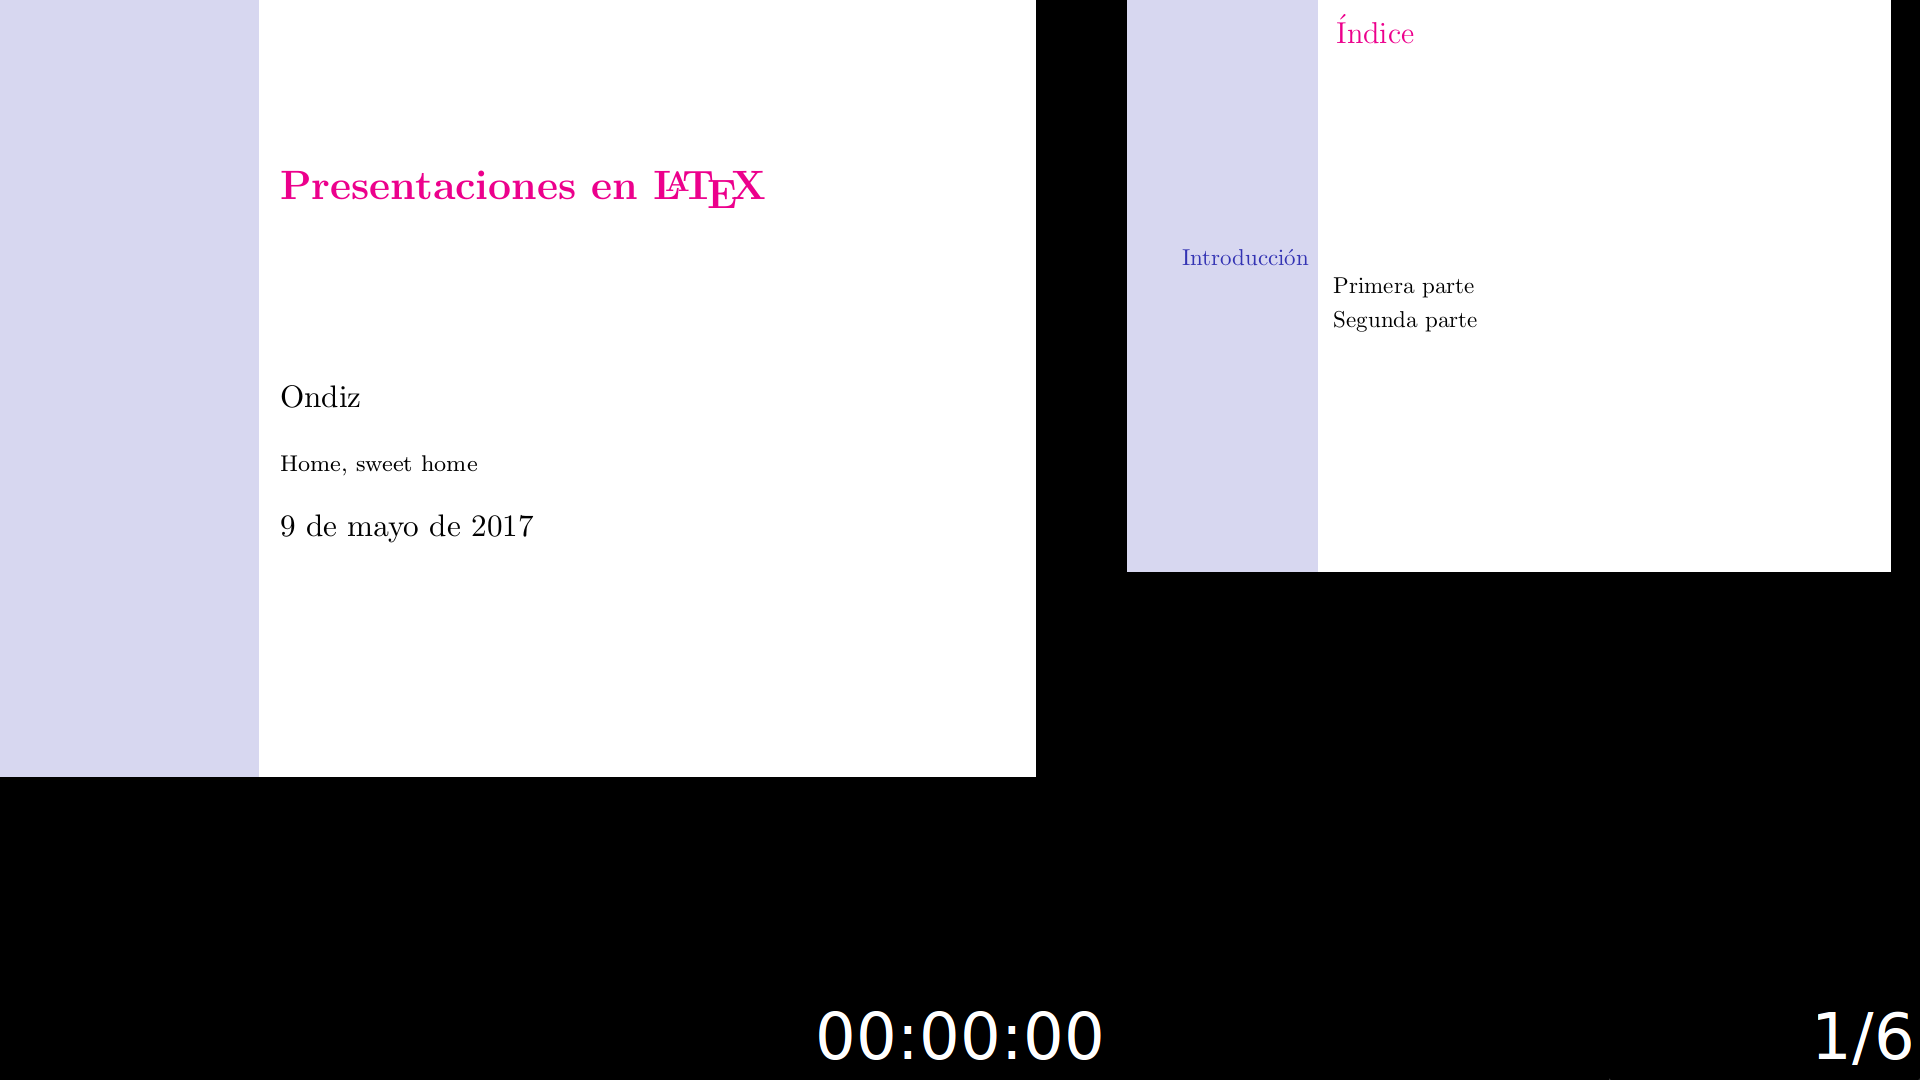
\includegraphics[width=\textwidth]{docs/Figuras/pdfpc.png}
\caption{pdfpc en acción}
\end{figure}

Para ver las notas de \lstinline!beamer! necesitamos crear la
presentación con las notas integradas como hemos visto antes:

\begin{lstlisting}
\setbeameroption{show notes on second screen=right}
\end{lstlisting}

Luego llamamos a \emph{pdfpc} con la opción \lstinline!--notes!:

\begin{lstlisting}[language=bash]
pdfpc presentation.pdf --notes=right
\end{lstlisting}

Ahora en la vista de presentador veremos las notas y una minidiapositiva
mostrándonos la diapositiva actual, en lugar de verla en grande como
antes.

\begin{figure}[htbp]
\centering
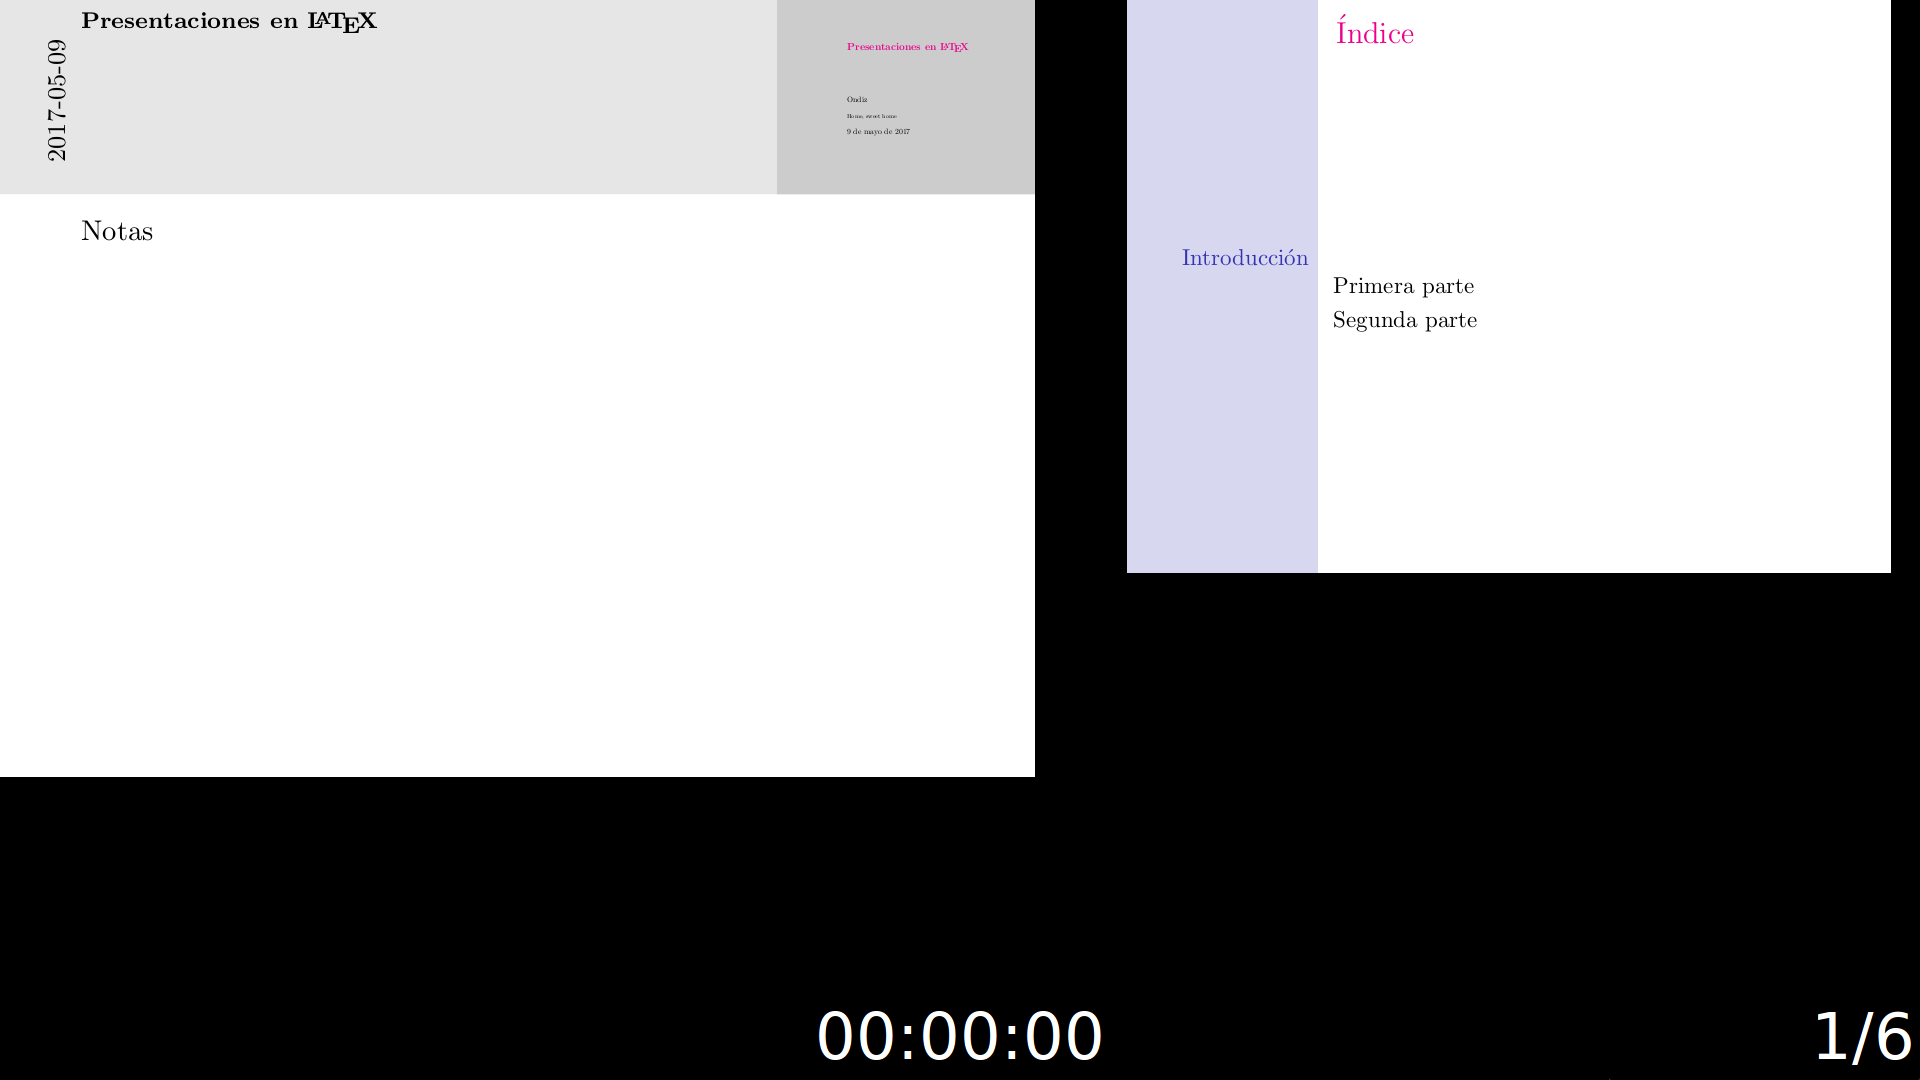
\includegraphics[width=\textwidth]{docs/Figuras/pdfpcNotas.png}
\caption{pdfpc con notas}
\end{figure}

El programa tiene otras muchas opciones, os resumo unas pocas que me
parecen especialmente útiles, las demás están en el manual:

\begin{itemize}
\item
  \lstinline!-d!, \lstinline!--duration=N! la duración en minutos
  (\lstinline!N!) de la presentación. Sirve para que nos ponga una
  cuenta atrás en la parte inferior de la pantalla.
\item
  \lstinline!-l!, \lstinline!--last−minutes=N! tiempo en minutos
  (\lstinline!N!) a partir del que la cuenta atrás se verá en rojo. Para
  irse poniendo nerviosillo.
\item
  \lstinline!-s!, \lstinline!--switch−screens! cambia la vista de
  presentador de pantalla.
\item
  \lstinline!-w!, \lstinline!--windowed! crea dos ventanas, una con la
  vista del presentador y otra con lo que verá la audiencia. Útil para
  ver el resultado cuando solo tenemos una pantalla.
\end{itemize}

Por ejemplo, para presentación de la tesis usé lo siguiente\footnote{Y
  no llegué a la cuenta atrás en rojo porque en media hora lo tenía
  ventilado.}:

\begin{lstlisting}[language=bash]
pdfpc presentation.pdf --duration=45 --notes=right --last-minutes=10
\end{lstlisting}

Además, durante la presentación se pueden usar diferentes teclas para
\emph{hacer cosas}:

\begin{itemize}
\item
  \lstinline!F! (\emph{freeze}): congela la imagen de la presentación
  para la audiencia mientras nosotros jugamos en nuestra vista. Pinta un
  copo de nieve en la parte inferior.
\item
  \lstinline!B! (\emph{black}): pone la pantalla de la audiencia negra y
  a nosotros nos pinta un cuadradito negro con una cruz blanca. Útil
  cuando das clase y alternas pizarra y proyector (así no montas el lío
  que solían montar mis profesores, ingenieros industriales casi todos
  ellos).
\item
  \lstinline!G! (\emph{go}): nos lleva a la diapositiva que le
  indiquemos. Fantástico para cuando te dicen \emph{en la diapositiva 12
  hay una tabla que\ldots{}}
\item
  \lstinline!N! (\emph{notes}): nos permite escribir notas en la
  diapositiva. Salimos con \lstinline!ESC!.
\item
  \lstinline!E! (\emph{end}): marca la diapositiva final. Útil si
  tenemos \emph{diapositivas de repuesto} para las preguntas.
\item
  \lstinline!O! (\emph{overlay}): sirve para marcar/desmarcar
  diapositivas como parte de una diapositiva que va surgiendo poco a
  poco. No las tendrá en cuenta en el cómputo total de diapositivas.
\item
  \lstinline!P! (\emph{pause}): pausa el reloj.
\item
  \lstinline!R! (\emph{reset}): reinicia la presentación.
\item
  \lstinline!Q! (\emph{quit}) o \lstinline!ESC!: cierra la presentación.
\end{itemize}

Las notas y diferentes marcas (fin, \emph{overlay}, \ldots{}) las guarda
en un archivo \emph{pdfpc} que recupera cada vez que leemos la
presentación. Es un archivo de texto plano y podemos abrirlo. Tiene esta
pinta:

\begin{lstlisting}
[file]
presentation.pdf
[duration]
45
[skip]
8,
[end_user_slide]
10
[notes]
### 1
Notas en la diapositiva 1
\end{lstlisting}

\subsection{Otras opciones para
presentar}

Los programas que cito ahora nunca los he usado, encontré \emph{pdfpc} y
me quedé con él, los pongo aquí para que vosotros elijáis el que más os
guste.

\begin{itemize}
\item
  \href{http://impressive.sourceforge.net/}{\emph{Impressive}}\footnote{¡Gracias
    a \href{https://quitter.se/notice/9129937}{Shevek} por informarme de
    su existencia!}: un programa escrito en Python con funcionalidades
  curiosas como el modo foco y la vista global de todas las
  diapositivas.
\item
  \href{https://github.com/Cimbali/pympress}{\emph{Pympress}}: también
  escrito en Python, soporta vídeo y las notas de \lstinline!beamer! y
  tiene una consola para el presentador.
\item
  \href{https://github.com/dannyedel/dspdfviewer}{\emph{Dspdfviewer}}:
  un visor simple para las presentaciones de \lstinline!beamer!.
\end{itemize}

\section{Resumen}

Para resumir lo que hemos estado comentando, vamos a ver cómo quedaría
un ejemplo completo aunque sencillo de una presentación en LaTeX:

\begin{lstlisting}[language={[latex]tex}]
% Definición
\documentclass{beamer}

% Notas
\usepackage{pgfpages}
\setbeameroption{show notes on second screen=right}

% Datos
\title{Presentaciones en \LaTeX}
\author{Ondiz}
\institute{Home, sweet home}
\date{\today}

% Temas
\usetheme{Bergen}
\usefonttheme{serif}
\usecolortheme{rose}

% Opciones
\setbeamercolor{title}{fg=magenta, bg=white}
\setbeamertemplate{navigation symbols}{}

% Inicio
\begin{document}

% Diapositivas
 \begin{frame}
  \maketitle
  \note{Notas}
 \end{frame}
 
 \begin{frame}{Índice}
  \tableofcontents
  \note{Más notas}
 \end{frame}
 
 \section{Introducción}
 \subsection{Primera parte}

 \begin{frame}{Introducción}
  \begin{itemize}
   \item<1-> Ítem 1
   \item<2> Ítem 2
  \end{itemize}
 \end{frame}

\end{document}
\end{lstlisting}

¡No es tan difícil!

En cualquier caso, para empezar con \lstinline!beamer! yo recomendaría
coger una presentación ya hecha y probar a cambiar cosas hasta que nos
sintamos cómodos con este nuevo sistema de trabajo. Cuando ya manejemos
lo más sencillo ir al manual (o a StackOverflow) y personalizar la
presentación es coser y cantar.

Por último, como soy maja os dejo una presentación de
\href{https://github.com/Ondiz/cursoLatex/tree/master/Ejemplos/Presentacion}{ejemplo}
en el repositorio del curso, contiene muchas de las cosas que he
comentado.

\section{Referencias}

\href{https://tex.stackexchange.com/questions/16204/which-package-to-use-for-presentations-beamer-prosper-or-other}{\emph{Which
package to use for presentations? Beamer, Prosper, or Other} en
TeXExchange}

\href{http://www.dmi.me.uk/blog/2010/11/08/creating-a-presentation-with-latex-and-powerdot/}{\emph{Creating
a presentation with LaTeX and powerdot}}

\href{http://osl.ugr.es/CTAN/macros/latex/contrib/beamer/doc/beameruserguide.pdf}{Manual
de \lstinline!beamer!}

\href{https://tug.org/pracjourn/2005-2/miller/miller.pdf}{\emph{Producing
beautiful slides with LaTeX}}

\href{https://hartwork.org/beamer-theme-matrix/}{\emph{Beamer theme
matrix}}

\href{http://www.deic.uab.es/~iblanes/beamer_gallery/index.html}{\emph{Beamer
theme gallery}}

\href{https://www.r-bloggers.com/create-your-own-beamer-template/}{\emph{Create
your own beamer template}}

\href{https://tex.stackexchange.com/questions/1574/embedding-videos-and-animations}{\emph{Embedding
videos and animations} en TeXExchange}

\href{https://tex.stackexchange.com/questions/21777/is-there-a-nice-solution-to-get-a-presenter-mode-for-latex-presentations}{\emph{Is
there a nice solution to get a ``presenter mode'' for Latex
presentations?} en TeXExchange}
